%%%%%%%%%%%%%%%%%%%%%%%%%%%%%%%%%%%%%%%%%
% Beamer Presentation
% LaTeX Template
% Version 1.0 (10/11/12)
%
% This template has been downloaded from:
% http://www.LaTeXTemplates.com
%
% License:
% CC BY-NC-SA 3.0 (http://creativecommons.org/licenses/by-nc-sa/3.0/)
%
%%%%%%%%%%%%%%%%%%%%%%%%%%%%%%%%%%%%%%%%%

%----------------------------------------------------------------------------------------
%	PACKAGES AND THEMES
%----------------------------------------------------------------------------------------

\documentclass{beamer}

\mode<presentation> {

% The Beamer class comes with a number of default slide themes
% which change the colors and layouts of slides. Below this is a list
% of all the themes, uncomment each in turn to see what they look like.

% \usetheme{default}
%\usetheme{AnnArbor}
%\usetheme{Antibes}
% \usetheme{Bergen}
%\usetheme{Berkeley}
%\usetheme{Berlin}
%\usetheme{Boadilla}
% \usetheme{CambridgeUS}
%\usetheme{Copenhagen}
%\usetheme{Darmstadt}
%\usetheme{Dresden}
% \usetheme{Frankfurt}
%\usetheme{Goettingen}
%\usetheme{Hannover}
%\usetheme{Ilmenau}
%\usetheme{JuanLesPins}
%\usetheme{Luebeck}
\usetheme{Madrid}
%\usetheme{Malmoe}
%\usetheme{Marburg}
%\usetheme{Montpellier}
%\usetheme{PaloAlto}
%\usetheme{Pittsburgh}
%\usetheme{Rochester}
%\usetheme{Singapore}
%\usetheme{Szeged}
%\usetheme{Warsaw}

% As well as themes, the Beamer class has a number of color themes
% for any slide theme. Uncomment each of these in turn to see how it
% changes the colors of your current slide theme.

%\usecolortheme{albatross}
%\usecolortheme{beaver}
%\usecolortheme{beetle}
%\usecolortheme{crane}
%\usecolortheme{dolphin}
%\usecolortheme{dove}
%\usecolortheme{fly}
%\usecolortheme{lily}
%\usecolortheme{orchid}
%\usecolortheme{rose}
%\usecolortheme{seagull}
%\usecolortheme{seahorse}
%\usecolortheme{whale}
%\usecolortheme{wolverine}

%\setbeamertemplate{footline} % To remove the footer line in all slides uncomment this line
%\setbeamertemplate{footline}[page number] % To replace the footer line in all slides with a simple slide count uncomment this line

%\setbeamertemplate{navigation symbols}{} % To remove the navigation symbols from the bottom of all slides uncomment this line
}

\usepackage{graphicx} % Allows including images
\usepackage{booktabs} % Allows the use of \toprule, \midrule and \bottomrule in tables
\usepackage{listings}

\lstdefinestyle{customjava}{
  breaklines=true,
  frame=L,
  xleftmargin=\parindent,
  language=Java,
  showstringspaces=false,
  basicstyle=\footnotesize\ttfamily,
  keywordstyle=\bfseries\color{green!40!black},
  commentstyle=\itshape\color{gray!40!black},
  identifierstyle=\color{blue},
  stringstyle=\color{orange},
}

\lstdefinestyle{customc}{
  breaklines=true,
  frame=L,
  xleftmargin=\parindent,
  language=[sharp]C,
  showstringspaces=false,
  basicstyle=\footnotesize\ttfamily,
  keywordstyle=\bfseries\color{green!40!black},
  commentstyle=\itshape\color{gray!40!black},
  identifierstyle=\color{blue},
  stringstyle=\color{orange},
}
%----------------------------------------------------------------------------------------
%	TITLE PAGE
%----------------------------------------------------------------------------------------

\title[Layered network architecture]{Layered network architecture} % The short title appears at the bottom of every slide, the full title is only on the title page

\author{Jonathan Windle} % Your name
\institute[UEA] % Your institution as it will appear on the bottom of every slide, may be shorthand to save space
{
University of East Anglia \\ % Your institution for the title page
\medskip
\textit{J.Windle@uea.ac.uk} % Your email address
}
\date{\today} % Date, can be changed to a custom date7

\begin{document}

\begin{frame}
\titlepage % Print the title page as the first slide
\end{frame}

\begin{frame}[allowframebreaks]
\frametitle{Overview} % Table of contents slide, comment this block out to remove it
\tableofcontents % Throughout your presentation, if you choose to use \section{} and \subsection{} commands, these will automatically be printed on this slide as an overview of your presentation
\end{frame}
%-----------------------------------------------------------------------
\section{Communication Network topology}
\begin{frame}
\frametitle{Communication Network topology}
\begin{itemize}
\item The {\color{red} topology} of a network is the connectivity of the {\color{green} nodes} in a network.
\item A number of physical {\color{red} topologies} are possible dependant on the underlying network technology.
\item But to an application point of view, it should be a fully connected graph
\item That is, a process should be able to use a service by:\\
\texttt{\color{orange}SEND(machine4,Process2,MyMessage)}\\
and not be concerened how the message is sent.
\item Enables the application to consider all machines as being connected to all machines. 
\item Routing, reliability etc is kept away from applications.
\item The physical connection can be very complex and vary dramatically, but the application does not care.
\end{itemize}
\end{frame}
%-------------------------------------------------------------------------
\section{Protocol Hierarchies}
\begin{frame}[allowframebreaks]
\frametitle{Protocol Hierarchies}
\begin{itemize}
\item To reduce {\color{red} complexity} networks are typically arranged in terms of layers.
\item Each layer has its own functions to perform.
\item Number, functionality and content of each layer varies for different designs of network.
\item Layer $n$ on one machine converses with layer $n$ on the other machine.
\item These are {\color{green}layer $n$ protocols}.
\end{itemize}
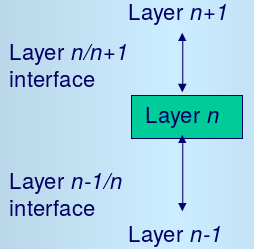
\includegraphics[scale=0.4]{lay.png}
\begin{itemize}
\item Entities comprising corresponding layers on each machine are {\color{purple}peers}. 
\item {\color{purple}Peers} communicate using a {\color{orange}protocol}.
\item No data is transferred directly between layer $n$ on one machine to layer $n$ on the other.
\item Data must go through the full stack of layers across the transfer medium and then up the stack on the other side.
\end{itemize}
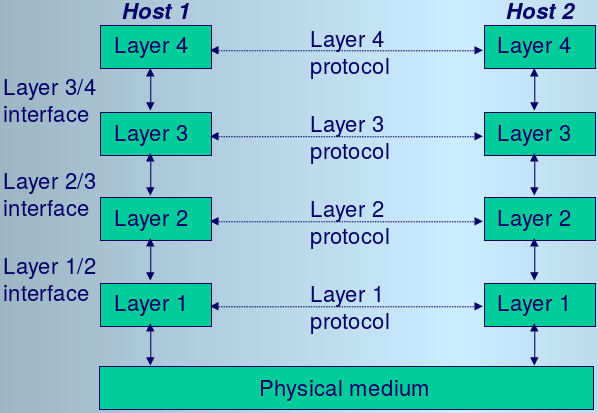
\includegraphics[scale=0.3]{flayer.png}
\begin{itemize}
\item Interfaces define the operation and services available to the next layer.
\item The set of layers and protocols is called {\color{magenta} Network Architecture}.
\item The specification must contain sufficient details to allow developers to write applications that obey defined protocols.
\item The list of protocols is called the {\color{blue} Protocol stack}.
\end{itemize}
\end{frame}
%-----------------------------------------------------------------------------
\subsection{Design Considerations}
\begin{frame}
\frametitle{Design Considerations}
\small
\begin{itemize}
\item \textbf{Addressing:} Needs a form of adressing to locate individual computers communicating over it to identify themselves and processes/applications.
\item \textbf{Data Transfer:} Various rules for data transfer. Network may only be able to offer \textit{simplex} connection, whereas others may be \textit{half-duplex} or \textit{full-duplex}.
\item \textbf{Error Control:} Need agreed error detection/correction due to instable physical networks.
\item \textbf{Sequencing:} Packet order might not be preserved. Need to allow receiver to restore original order. Could involve packet numbering/timestamping.
\item \textbf{Data rates:} Sender/Receiver may not be matched in terms of capacity. Need a facility to control flow of data so fast sender does not overload slow receiver.
\item \textbf{Long messages:} Some are restricted in terms of the maximum size a message can be, may need to segment into smaller messages and restructure the other side.
\item \textbf{Routing:} Decision on which route to take based on factors such as cost, current network traffic etc.
\end{itemize}
\end{frame}
%-------------------------------------------------------------------------------------
\section{Reference models}
\subsection{ISO OSI Reference Model}
\begin{frame}[allowframebreaks]
\frametitle{ISO OSI Reference Model}
\begin{itemize}
\item Has {\color{red} Seven} layers.
\item Each of the layers is required to exist even if the functionality of a layer is minimal or non-existent.
\end{itemize}
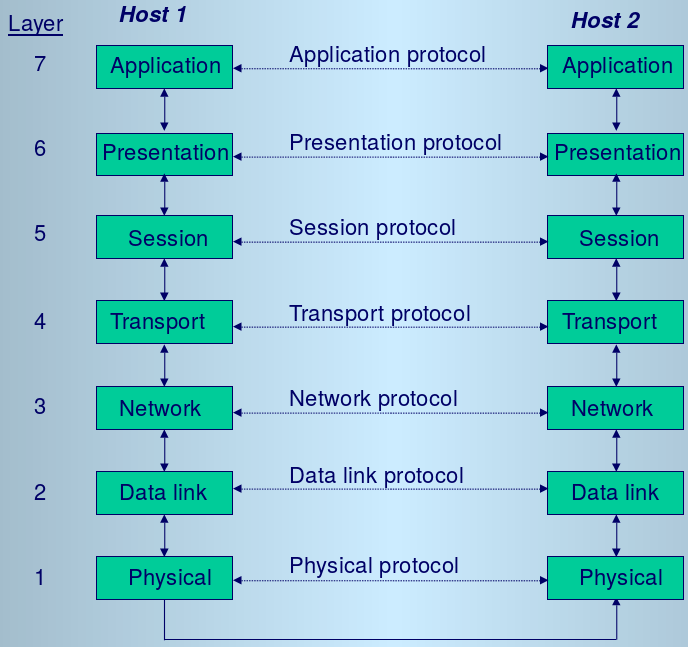
\includegraphics[scale=0.25]{osi.png}
\begin{enumerate}
\item \textbf{Physical layer:} Transmission of raw bits over a communication channel.
\item \textbf{Data link layer:} Takes raw binary transmission and transforms it into a more reliable channel. Introduces error detection and correction. Regulates flow of transmission. May segment data into smaller frames.
\item \textbf{Network layer:} Concerened with routing of packets from source to destination. Can be static or dynamic. Also concerned with congestion control.
\item \textbf{Transport layer:} Accepts from session layer and sends to network layer with responsibility of ensuring delivery. Also concerned with flow control and process addressing.
\item \textbf{Session layer:} Allows sessions to be established by users on different machines. May manage dialogue control- whose turn is it to communicate - token management. Also concerned with synchronization - insertion of sync points - useful for large file transfers.
\item \textbf{Presentation layer:} Concerned with encoding data in particular ways. Format for data such as names, dates, prices may be agreed in this layer. Convention integers, characters, byte-order etc too. Also compression and encryption.
\item \textbf{Application layer:} Variety of protocols which are commonly used. Include file transfer which may need to consider different conventions adopted on different machines.
\end{enumerate}
Data transmission occurs with each layer, sometimes adding its own header before being passed down to the next layer.\\
At the receiver, the headers are removed and sent up to the next layer.
\end{frame}
%----------------------------------------------------------------------------------
\subsection{TCP/IP Reference model}
\begin{frame}[allowframebreaks]
\frametitle{TCP/IP Reference Model}
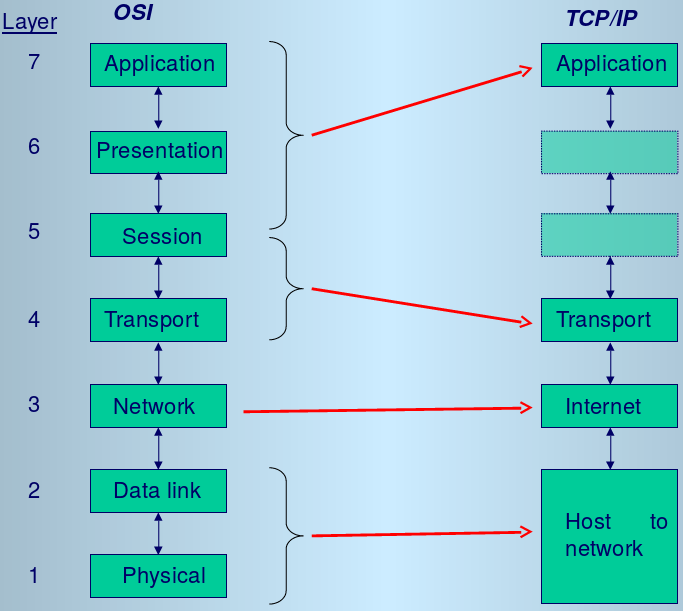
\includegraphics[scale=0.35]{tcp.png}
\begin{itemize}
\item \textbf{Host to Network layer:} Not particularly well defined. Host has to connect to the network in some way to deliver IP packets.
\item \textbf{Internet layer:} packet-switched and connectionless communication. Layer is concerned with delivering IP packets to their correct destination. Based around IP.
\item \textbf{Transport layer:} Allows peer entities on different machines to communicate with each other. Two protocols available TCP (Transmission Control Protocol) and UDP (User Datagram Protocol). TCP is reliable and connection-orientated. UDP is unreliable and connectionless.
\item \textbf{Application layer:} Contains higher layer protocols. No session or presentation layers. Examples are FTP, SMTP and  DNS.
\end{itemize}
\end{frame}
%---------------------------------------------------------------------------------
\subsection{Tanenbaum Hybrid Reference Model}
\begin{frame}
\frametitle{Tanenbaum Hybrid Reference Model}
\begin{columns}[c]
\column{.2\textwidth}
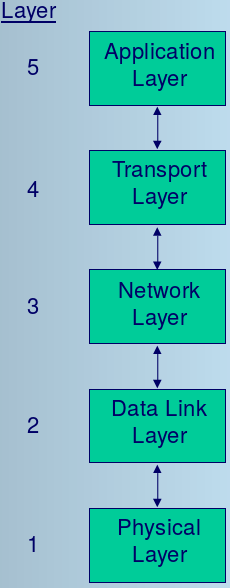
\includegraphics[scale=0.3]{tan.png}
\column{.8\textwidth}
\begin{itemize}
\item Hybrid model based on a modified OSI 7 layer model, but designed to concentrate mainly on the TCP/IP protocols.
\end{itemize}
\end{columns}
\end{frame}
%----------------------------------------------------------------------------------
\begin{frame}
\Huge{\centerline{The End}}
\end{frame}

%----------------------------------------------------------------------------------------

\end{document}